\documentclass[twocolumn]{article}
\usepackage[utf8]{inputenc}
\usepackage{graphicx}


\title{Exponential function}
\author{Marta Lønne Jensen}
\date{\today}

\begin{document}
\maketitle

\section{Introduction}

The exponential function is a function denoted by

\begin{equation}
	\exp(x) = e^x
\end{equation}

The inverse of the exponential function is the natural logarithm, $\ln(x)$.
\section{Implementation}

This report uses a "quick and dirty" implementation of the exponential function, given as

\begin{equation}
\label{eq:imp}
	f(x) = 1 + x + \frac{x^2}{2} + \frac{x^3}{3} + ... + \frac{x^{10}}{10}
\end{equation}



\section{Test}

As can be seen in fig. \ref{fig:exp}, the implementation is working.

\begin{figure}
	\label{fig:exp}
	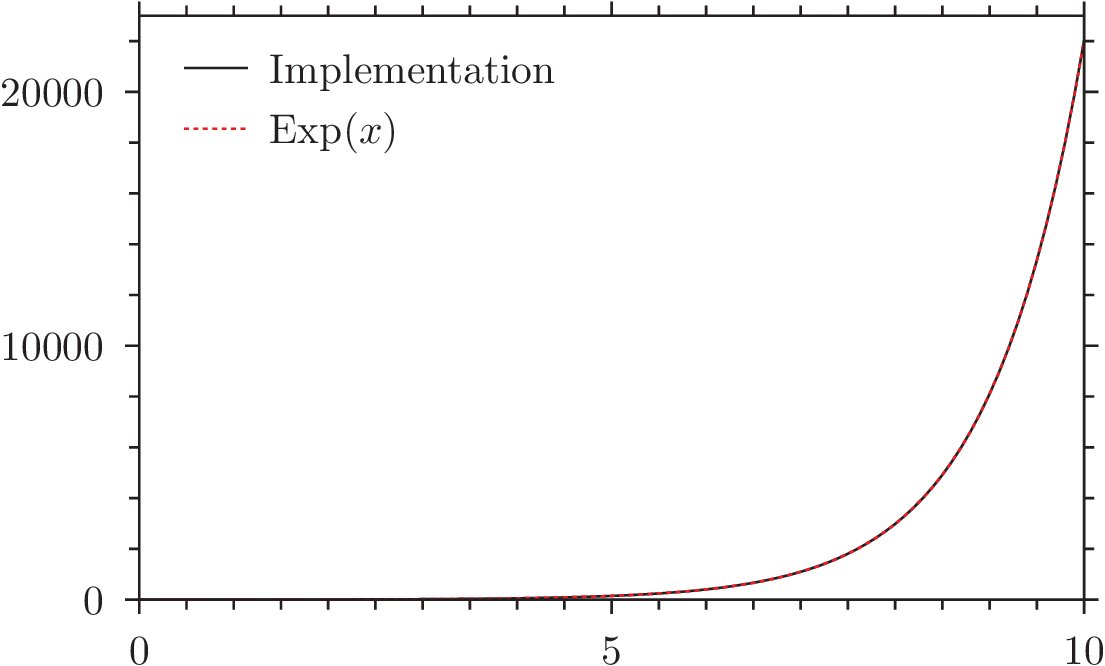
\includegraphics{exp.png}
	\caption{Implementation of eq. (\ref{eq:imp}).}
\end{figure}
\end{document}
